\lecture{7}{2025-03-10}{ Logic Synthesis}{}
\subsection{Logic synthesis}
\begin{parag}{Minterms}
    For a function $f = (x_1, x_2, \dots, x_n)$ of $n$ variables, a \important{product term} in which \important{each} of the $n$ variables appears \important{once} is called a \important{minterm}.\\
    Minterms are typically labeled as $m_i$, where $i \geq 0$ is an integer. An $n-$variable minterm $m_i$ can be represented by an $n$-bit integer. 
    \begin{itemize}
        \item Variable appears \important{complemented} if the corresponding bit in the binary representation of $m_i$ is $0$
        \item Otherwise, it appears \important{uncomplemented} (original)
    \end{itemize}
    \begin{subparag}{Example}
        Let us take $n = 3, i = 5$: three variables. $5 = 101_2$ and therefore, $m_5 = x_1 \overline{x_2}x_3$\\
        If we take now $n = 5, i = 3$: five variables. $3 = (00011)_2$ and therefore, $m_3 = \overline{x_1} \overline{x_2} \overline{x_3} x_4 x_5$
       
        
    \end{subparag}
\end{parag}
\begin{parag}{Maxterms}
    For a function $f = (x_1, x_2, \dots, x_n)$ of $n$ variables, a \important{sum term}
 in which \important{each} of the $n$ variables appears \important{once} is called a \important{maxterm}. Maxterm are typically labeled as $M_i$, where $i \geq 0$ is an integer. An $n-$variable maxterm $M_i$ can be represented by an $n-$bit intgerer.
 \begin{itemize}
     \item Variable appears \important{complemented} if the corresponding \important{bit} in the binary representation of $M_i$ is $1$.
     \item Othewise, it appears \important{uncomplemented} (original)
 \end{itemize}
 \begin{subparag}{Example}
     if we take the same as above, $n = 3, i = 5$ with $5 = 101_2$ we get:
     \begin{align*}
         M_5 = \overline{x_1} + x_2 + \overline{x_3}
     \end{align*}
     And as we take the second way, $n=5, i = 3$ we get:
     \begin{align*}
         x_1 + x_2 + x_3 + \overline{x_4} + \overline{x_5}
     \end{align*}
 \end{subparag}
 \begin{framedremark}
     What we are doing here is the same thing as seen in AICC I, we use it the same way as CNF and DNF where one is with negation on the  $1$ and the \textit{OR} between each variable and the other with \textit{AND} everywhere but the opposite.
     \\
     This is equivalent because of the Morgan's law.
 \end{framedremark}
 
\end{parag}  


\begin{parag}{Logic synthesis with Minterm/Maxterms}
    For a function $f$ specified in the form of a truth table, a logic expression realizing the function can be obtained by considering:
    \begin{itemize}
        \item Only the rows in the table for which $f = 1$ or
        \item Only the rows in the table for which $f = 0$
    \end{itemize}

    If we are considering the rows where \important{$f = 1$}, $f$ is represented by the \important{sum of the minterms} corresponding to the rows where $f = 1$. \\
If we are considering the rows where \important{$f = 0$}, $f$ is decribed by \important{the product of the maxterms} corresponding to the rows where $f = 0$
\end{parag}

\begin{parag}{Sum of products (SoP) form}
   When we are considering the rows where $f = 1$, f is represented by the sum of the corresponding minterms. The resulting logical expression is correct but \textbf{not} necessarily the lowest cost (optimal) implementation of $f$. \\
   Any logical expression consisting of product (AND) terms that are summed (OR) is said to be in the \important{sum-of-products (SoP)} form.
   \begin{definition}
       We called the \important{canonical sum of products} where all the product are a minterm
   \end{definition}
   
 \begin{subparag}{Example SoP}
     Consider a function $f$ of $ n = 3$ variables and the truth table below:
     \begin{center}
     \begin{tabular}{ccc|c}
         \hline
         $x_1$ & $x_2$ & $x_3$ & $f$ \\
         \hline
         \hline
         0 & 0 & 0 & 0 \\
         \hline
         0 & 0 & 1 & 1\\
         \hline
         0 & 1 & 0 & 0 \\
         \hline
         0 & 1 & 1 & 0 \\
         \hline
         1 & 0 & 0 & 1 \\
         \hline
         1 & 0 & 1 & 1 \\
         \hline
         1 & 1 & 0 & 1 \\
         \hline
         1 & 1 & 1 & 0 \\
         \hline
     \end{tabular}
     \end{center}
    Then, the canonical  SoP form:
    \begin{align*}
        f(x_1, x_2, x_3) &= \sum(m_1, m_4, m_5, m_6) \\
                         &= \sum m(1, 4, 5, 6)
    \end{align*}
    \begin{align*}
        f(x_1, x_2, x_3) &= \overline{x_1} \overline{x_2} x_3 + x_1 \overline{x_2} \overline{x_3} + x_1 \overline{x_2} x_3 + x_1 x_2 \overline{x_3} \\
                         &= \overline{x_2} x_3 + x_1 \overline{x_3}
    \end{align*}
    Which get us to:
    \begin{center}
    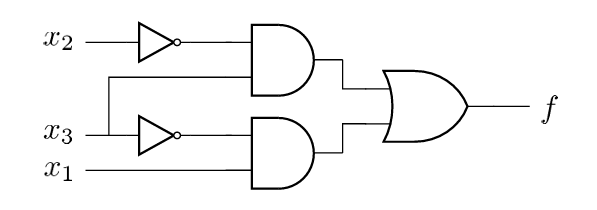
\includegraphics[scale=0.6]{logicgate2025-03-10.png}
\end{center} 
    A good indication of the \important{cost} of a logic circuit is the total number of \textbf{gates} and the \textbf{input} to the gates in the circuit.
    \begin{itemize}
        \item For the design above, the cost $ = 5 + 1 + 1 + 2 + 2 + 2 = 13$ where $5$ is the total gates, the one's are the NOT, $2$'s are the AND and OR.
            
    \end{itemize}
 \end{subparag}
 \begin{subparag}{Example PoS}
     Now we consider with product instead of a sum. Consider a function $f$ of $n = 3$ variables and the truth table below:
     \begin{align*}
         f(x_1, x_2, x_3) &= \prod(M_0, M_2, M_3, M_7) \\
                          &= \prod M(0, 2, 3, 7)
     \end{align*}
     \begin{align*}
         f(x_1, x_2, x_3) &= M_0 \cdot M_2 \cdot M_3 \cdot M_7 \\
                          &= (x_1 + x_2 + x_3)(x_1 + \overline{x_2} + x_3)(x_1 + \overline{x_2} + \overline{x_3})( \overline{x_1} + \overline{x_2} + \overline{x_3})
     \end{align*}
     And now using the Morgan's theorem:
     \begin{align*}
         f = \overbrace{f}^{=}= \overline{m_0 + m_2 + m_3 + m-7}
     \end{align*}
      \begin{center}
     \begin{tabular}{ccc|c}
         \hline
         $x_1$ & $x_2$ & $x_3$ & $f$ \\
         \hline
         \hline
         0 & 0 & 0 & 0 \\
         \hline
         0 & 0 & 1 & 1\\
         \hline
         0 & 1 & 0 & 0 \\
         \hline
         0 & 1 & 1 & 0 \\
         \hline
         1 & 0 & 0 & 1 \\
         \hline
         1 & 0 & 1 & 1 \\
         \hline
         1 & 1 & 0 & 1 \\
         \hline
         1 & 1 & 1 & 0 \\
         \hline
     \end{tabular}
     \end{center}
     Which as you can see is the same as the one before, but now we only take the line with $0$ as a result.
     \\
     After some trick, we finally get the result:
     \begin{align*}
         f(x_1, x_2, x_3) =(x_1 + x_3)( \overline{x_2} + \overline{x_3})
     \end{align*}
     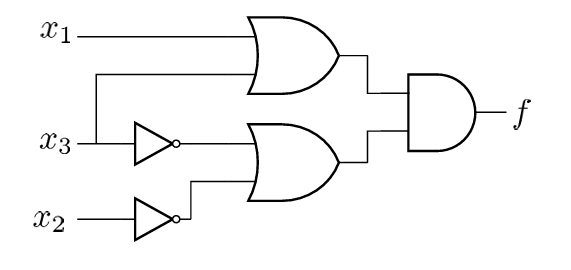
\includegraphics[scale=0.6]{gateAnd2025-03-10.png}
     Where the cost $ = 5 +  1 + 1 + 2 + 2 + 2 = 13$
 \end{subparag}
\end{parag}

\subsection{NANS and NOR logic Networks}
\begin{parag}{NAND and NOR gates}
    NAND and NOR gates can be used to build logic circuits:
    \begin{center}
        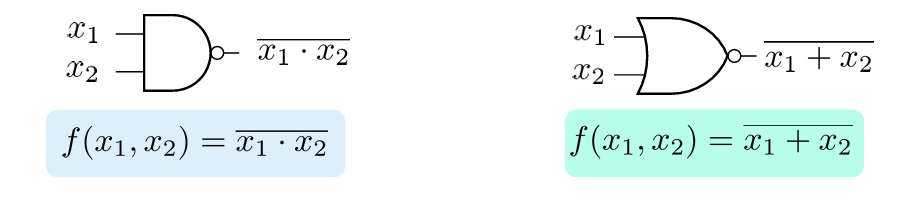
\includegraphics[scale=0.7]{NANDNOR2025-03-10.png}
    \end{center}
        NAND/NOR physical implementation is simpler (requires fewer transistor) and more efficient than AND/OR. In fact the AND and OR logic gates are implemented as NAND/NOR + not. How to de we that?:
        \begin{center}
            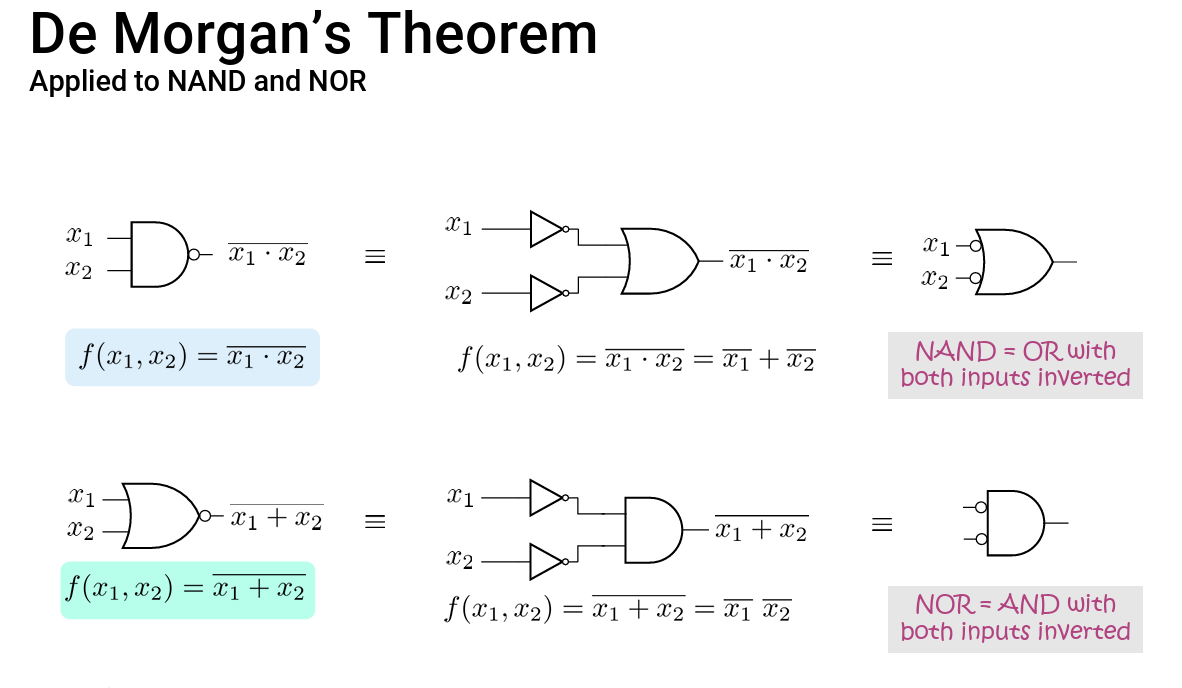
\includegraphics[scale=0.4]{morgantheoremgate2025-03-10.png}
        \end{center}

\end{parag}
\begin{parag}{NOT gate using NAND or NOR}
        According to Boolean theorems, $ \overline{x} = \overline{x \cdot x}$ and $ \overline{x} = \overline{x + x}$ which are the $NAND$ and the $NOR$:
\begin{center}
    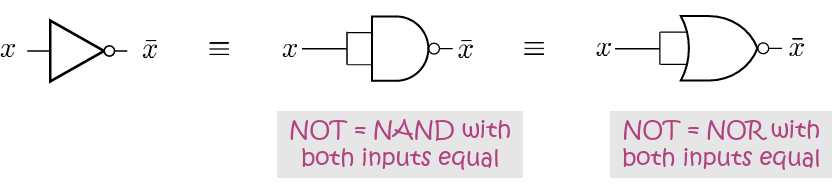
\includegraphics[scale=0.6]{notgatenandnor2025-03-10.png}
\end{center}
\begin{subparag}{How to implement a function}
    Now we try to implement the function $f$ in the $SoP$ form with $NAND$
    \begin{align*}
        f = x_2 + x_1 \overline{x_3}
    \end{align*}
    \textbf{Algorithm}: we start by applying double inversion and, then, the Morgan's theorem to simplify the expression.
    \\
    We have:
    \begin{align*}
        f &= x_2 + x_1 \overline{x_3} \\
          &= \overline{ \overline{ x_2 + x_1 \overline{x_3}}} \\
          &= \overline{ \overline{x_2} \cdot \overline{ x_1 \overline{ x_3}}}
    \end{align*}
    Which gives us:
    \begin{center}
        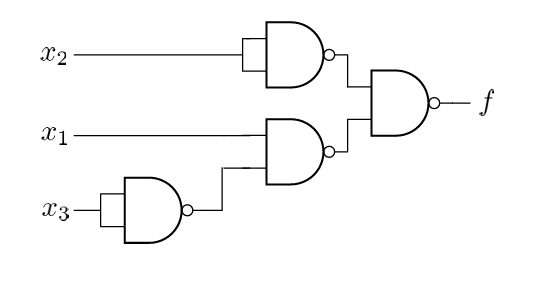
\includegraphics[scale=0.6]{gate22025-03-10.png}
    \end{center}
\end{subparag}

\end{parag}

\subsection{Incomplety definded Functions}
\begin{parag}{Incompletely defined function}
    …are Boolean functions where some input combinations are not specified because they don’t matter (e.g., they never occur), so the function does not need to define outputs for them
    \begin{itemize}
        \item Those input combinations are called \important{don't care conditions}
    \end{itemize}
    In logic optimization, don't care conditions can be assigned function value (output) either $0$ or $1$, to simplify the logic circuit
\end{parag}
\begin{parag}{Example}
    Imagine a lion's cage with an automated door control system including two sensors and a manual override switch.
    \textbf{Input}:
    \begin{itemize}
        \item \textbf{Sensor L} detects if the lion is inside ($1 =$ inside, $0 = $ outside=
        \item \textbf{Sensor T} detects if the trainer is inside ($1 = $ inside; $0 = $outside)
        \item \textbf{Override switch (S)}: The trainer can manually force the door open or closed irrespective of presence $(1 = $ override enabled; $0 = $ normal mode)
    \end{itemize}
    \textbf{Outputs}
    \begin{itemize}
        \item \textbf{Door control} $1$ = open, 0 = closed.
    \end{itemize}
    In this case with si that when $S = 1$ then L and $T$ doesn't matter, because the door will be open in any case.\\
    What we are doing here is this:
    \begin{align*}
        D = \overline{L}T \overline{S} + LT \overline{S} + \overline{L} \overline{T}S  = T \overline{S} + \overline{L} \overline{T}S
    \end{align*}
    Which have a cost of $ 3 + 7 = 10$\\
    However the result is the same by switching to
    \begin{align*}
        D = T + S
    \end{align*}
    In spoken english this is saying, the door can only be open if the switch is on or the trainer is inside and if neither of those two are true, then the door is closed. Here the cost is $1 + 2 = 3$
\end{parag}

\begin{parag}{Even and Odd detectors}
    Given the function $f = \overline{x_1}x_2 + x_1 \overline{x_2}$ which we called \important{Exclusive OR} or $XOR$ writted as $\oplus$:
    \begin{align*}
        f = x_1 \oplus x_2
    \end{align*}
    \begin{center}
        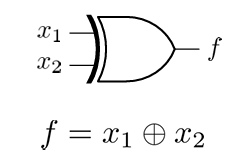
\includegraphics[scale=0.8]{xor2025-03-10.png}
    \end{center}
    On the other side for the $XNOR$ which is defined as $f = \overline{x_1} \overline{x_2} + x_1x_2$
    \begin{center}
        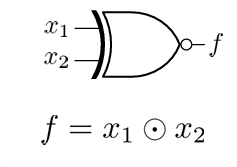
\includegraphics[scale=0.8]{xnor2025-03-10.png}
    \end{center}
    
\end{parag}
\begin{parag}{Number display}
    I skipped the previous slides (number display) because I am late but the goal was to write on a digital clock (with the 8 which as 7 lines that can be on or off) a value $(s_1, s_0)_2$ as a decimal number. To do so you have to do first a truth table depending of which line is on depending of the values, and the create a logic function from this truth table.
\end{parag}
\begin{parag}{Data selector}
    It is often helpful to choose \important{precisely one} from several inputs. A circuit performing data selection (a \important{multiplixer}) has one or more \important{select} inputs dedicated to determining which of the remaining inputs to pass to the output. \\
    For example, a three input multiplixer (also called $2$ to $2$ $MUX$):\\
    \textbf{Inputs}
    \begin{itemize}
        \item One \important{selection} signal $s$
        \item Two data \important{input} $x_1$ and $x_2$
    \end{itemize}
    When the selection signal is $s = 0$ the output becomes $f = x_1$ otherwise, the output becomes $f = x_2$\\
    To write this as a logical function:
\begin{align*}
    f(s, x_1, x_2) &= \overline{s}x_1 \overline{x_2} + \overline{s}x_1x_2 + s \overline{x}_1x_2 + sx_1x_2 \\
    \overline{s}x_1 ( \overline{x_2} + x_2) + s( \overline{x_1} + x_1)x_2 \\
    &= \overline{s}x_1 + sx_2
\end{align*}

\begin{subparag}{Remark}
  If there are $n$ data inputs to select from, how many select signals MUX requires?:
  \begin{align*}
      \left\lceil \log_2 n \right\rceil
  \end{align*}
  Because if we have two data, this give only one combination, 4 data two select signal, $2^2$, with eight data inputs, three select signals ($2^3$ combinations) and because we cannot take lower bound for data input that are not power of $2$, we have to take the ceiling.
  
\end{subparag}

\end{parag}




